\documentclass[a4paper,11pt]{article}
\usepackage[utf8]{inputenc}
\usepackage{amsmath}
\usepackage{graphicx}
\usepackage{subcaption}
\usepackage{float}
\usepackage{geometry}
\geometry{margin=1in}

\title{SH1017 Physics for Engineering Mathematics Lab 1}
\author{Lucas Frykman}
\date{\today}

\begin{document}

\maketitle

\section*{Q1: Period of Undamped Pendulum}

\textbf{Method:} We calculate the period $T$ of oscillation for different initial angular displacements $\theta_0$ by simulating the differential equation $\ddot{\theta} + \omega_0^2 \sin(\theta) = 0$ using the 4th order Runge-Kutta (RK4) method (\texttt{pendulum.py}). The simulation detects turning points to find the half-period. We compare this to a small angle approximation, a power series expansion, and direct numerical integration.

\begin{figure}[H]
    \centering
    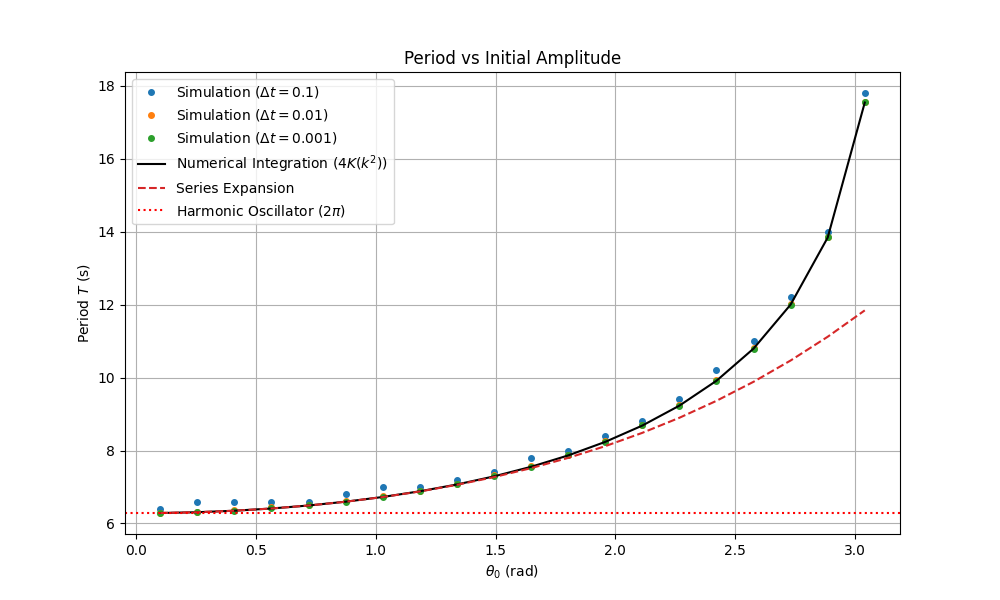
\includegraphics[width=\textwidth]{task1_period.png}
    \caption{Period $T$ as a function of the initial angular displacement $\theta_0$. Parameters: $\theta_0 \in [0.1, \pi - 0.1]$ (20 linearly spaced values), $\omega_0^2 = 1$. Time steps: $\Delta t \in \{0.1, 0.01, 0.001\}$.}
    \label{fig:period_vs_theta0}
\end{figure}
% \textbf{Theory:} For small initial angles, the pendulum behaves like a harmonic oscillator with a constant period $T = 2\pi$. For
% larger angles the restoring force is weaker than the linear approxiamtion $\theta$ which implies the period 
% should increase with amplitude. The power series expansion accounts for this but will eventually diverge
% from the true solution for very large angles. 

\textbf{Results:} We see in Figure 1 that all methods agree $T \approx 2\pi$ for angles near zero.
For larger angles, the period increases. The RK4 simulations for $\Delta t = 0.1$ to $\Delta t = 0.001$ coincides with the numerical integration. 
The series expanson gives an accurate approximation for angles below $\theta_0 \approx \pi/2$ as the angle approaches $\pi$.


\section*{Q2: Damped Pendulum}

\textbf{Method:} We simulate the damped pendulum equation $\ddot{\theta} + \gamma \dot{\theta} + \omega_0^2 \sin(\theta) = 0$ using RK4 
(\texttt{pendulum.py}). Using the data from the simulation, we plot the natural logarithm of the positive peak amplitudes vs time (this information is used to find the $\tau$ characteristic time).

% Since amplitude decays exponentially we have that $A(t)=A_0 e^{-\lambda t}$.
\begin{figure}[H]
    \centering
    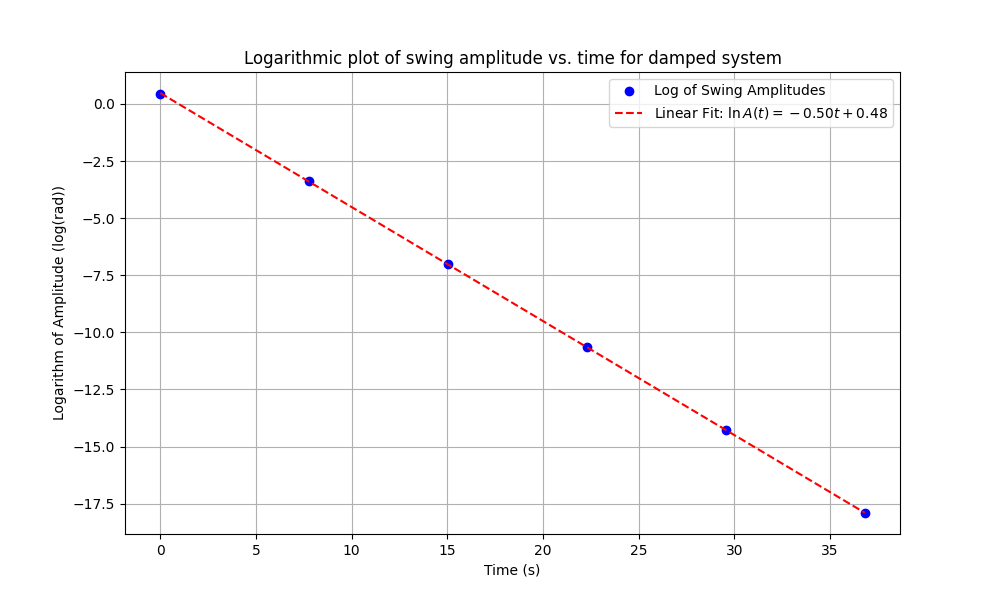
\includegraphics[width=\textwidth]{task2_log_fit.png}
    \caption{Logarithmic plot of swing amplitude vs. time for the damped system. Parameters: $\theta_0 = \pi/2$, $\gamma = 1.0$, $\omega_0^2 = 1$, $\Delta t = 0.01$, $t_{\text{max}} = 40$.}
\end{figure}

\begin{figure}[H]
    \centering
    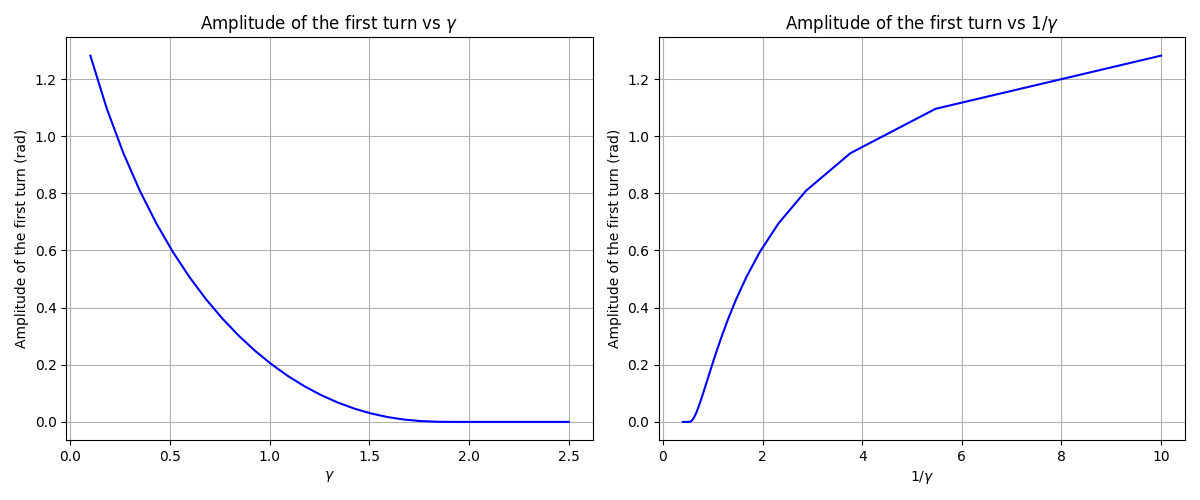
\includegraphics[width=\textwidth]{task2_first_turn_comparison.png}
    \caption{Comparison of the first turn amplitude for varying values of $\gamma$ and $1/\gamma$. Parameters: $\theta_0 = \pi/2$, $\gamma \in [0.1, 2.5]$ (30 linearly spaced values), $\omega_0^2 = 1$, $\Delta t = 0.01$, $t_{\text{max}} = 20$.}
\end{figure}

\textbf{Theory:} A weakly damped harmonic oscillator experiences an exponential decay in its amplitude over time, $A(t) = A_0 e^{\lambda t}$. This implies that $\ln A(t)$ should decrease linearly with a slope of $\lambda$. 
This gives
\[
\ln(\theta(t)) = \ln A_0 + \lambda t
\]

To find the characteristic time \(\tau\) where the initial amplitude \(A_0\) is halved we first find \(\lambda\) 
through linear interpolation \(\lambda \approx \frac{\ln A_2 - \ln A_1}{t_2 - t_1}\) 
where \(A_2\) and \(A_1\) are distinct turning point amplitudes. Then we solve the equation
\[
\ln A_0 + \lambda \tau = \ln\Bigl(\frac{A_0}{2}\Bigr) = \ln A_0 - \ln 2
\]
\[
\Longleftrightarrow \tau = -\frac{\ln 2}{\lambda}
\]
Furthermore, as the damping coefficient $\gamma$ increases, 
the system transitions toward an overdamped state.
In the overdamped case, the pendulum should not oscillate or cross the 
equilibrium point, meaning its subsequent peak amplitude is zero.

\textbf{Results:} Figure 2 shows a strong linear relationship for $\ln A(t)$ vs time, confirming that 
the nonlinear pendulum's envelope amplitude decays exponentially.
The slope gives an estimated decay constant $\lambda \approx -0.50$, 
from which we calculate the characteristic time $\tau = \ln(2)/\lambda \approx 1.39$ s. Figure 3 demonstrates that as $\gamma$ increases, the amplitude of the first turn decreases. 
It reaches exactly zero at $\gamma = 2.0$ (critical damping).
\section*{Q3: Driven Damped Pendulum}

\textbf{Method:} We simulate the driven damped system $\ddot{\theta} + \gamma \dot{\theta} + \omega_0^2 \sin(\theta) = A \cos(\omega t)$ using RK4 (\texttt{pendulum.py}). We then measure the 
steady-state amplitude across various drive amplitudes $A$. We then generate a phase portrait ($\theta$ vs $p$) for a drive amplitude $A=1.0$ 
by discarding the initial transient segment.

\begin{figure}[H]
    \centering
    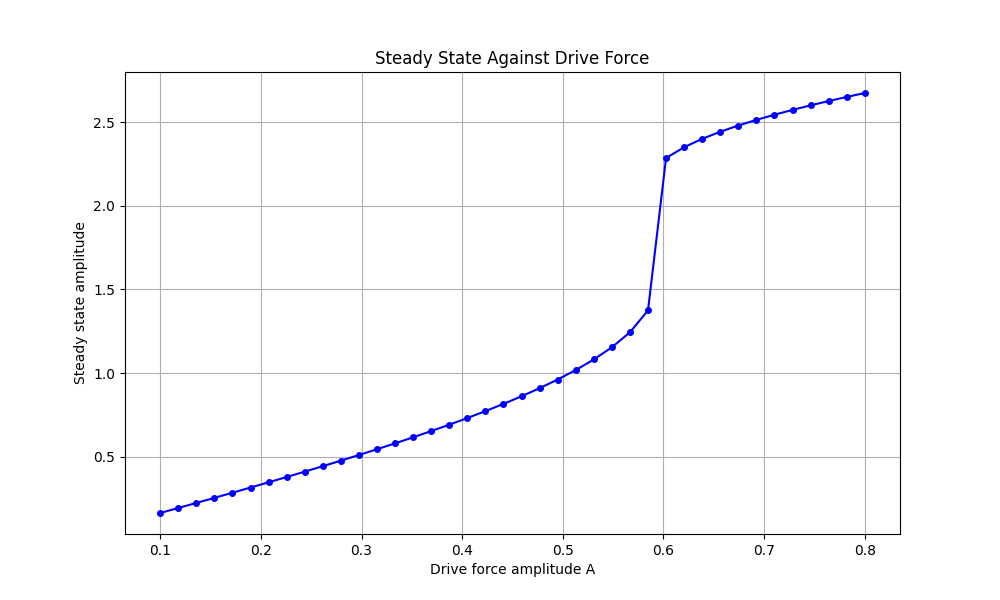
\includegraphics[width=\textwidth]{task3_steady_state_vs_A.png}
    \caption{Steady state amplitude against drive force amplitude $A$. Parameters: $\gamma = 3/8$, $\omega = 2/3$, $\omega_0^2 = 1$, $A \in [0.1, 0.8]$ (40 linearly spaced values), $\Delta t = 0.01$, simulated until $t = 1000$.}
\end{figure}

\begin{figure}[H]
    \centering
    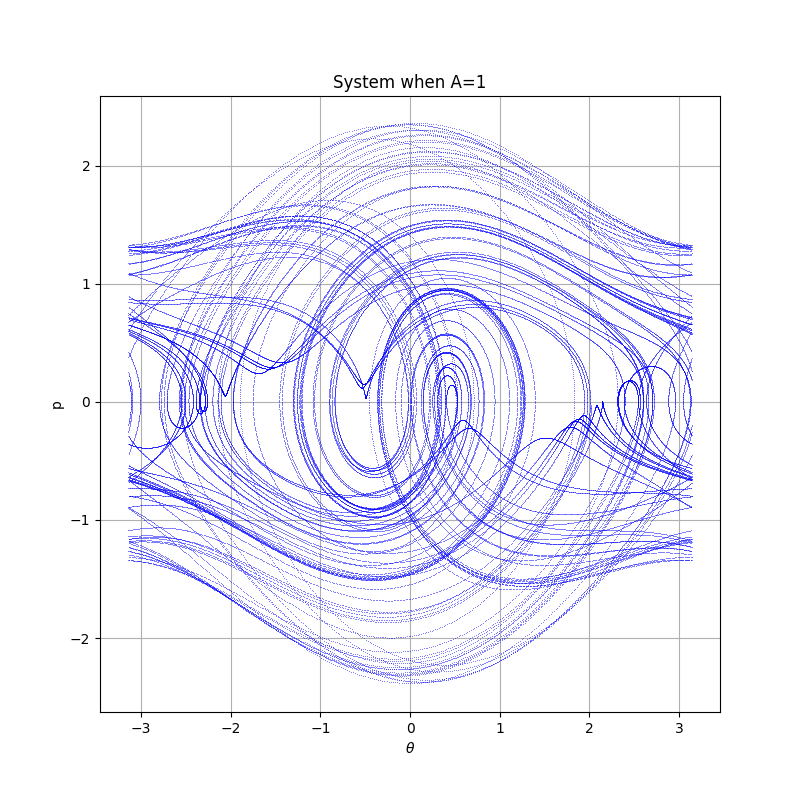
\includegraphics[width=\textwidth]{task3_A1_phase.png}
    \caption{Phase portrait of the system when $A=1$. Parameters: $\gamma = 3/8$, $\omega = 2/3$, $\omega_0^2 = 1$, $A = 1.0$, $\Delta t = 0.01$, simulated until $t = 1000$, transients discarded for $t < 200$.}
\end{figure}

% \textbf{Theory:} 
% The equation of motion here is given by:
% \[
% \ddot{\theta} = -\gamma \dot{\theta} - A \sin(\omega t) - \omega_0^2 \sin(\theta)
% \]

% We plot the steady state amplitude for different values of \(A\)
% \begin{align*}
% \theta_0 &= \dot{\theta}_0 = 0 \\
% \gamma &= 3/8 \\
% \omega &= 2/3 \\
% \omega_0 &= 1
% \end{align*}
\textbf{Results:}
The steady state amplitude is obtained by observing when the amplitude of the 
pendulum's position converges. It seems to only reach a steady state with 
small enough values of the drive force amplitude \(A\). If we imagine the 
turn amplitudes as a sequence namely \(X_1, X_2 \ldots X_k\), we stop at the 
amplitude such that \(|X_{k+1} - X_k| < \tau\) for a certain tolerance level 
\(\tau\). (See figure 4). We choose tolerance \(\tau = 1\mathrm{e}{-6}\). 
When the drive force amplitude is \(1 \leq A\), we find that the turn amplitude 
does not converge, i.e.\ the phase portrait does not reach a limit cycle. 
However, for $A=1$ the phase portrait does have periodic behavior as we can see in 
figure 5.
\end{document}
